\documentclass[article, hidelinks,oneside,12pt]{abntex2}

\usepackage{float} %fixar imagem
\usepackage[utf8]{inputenc} %língua
\usepackage{amsmath} %matemática
\usepackage{graphicx} %imagens
\usepackage{amssymb} %para adicionar laplace
\usepackage{indentfirst} %indentar primeiro parágrafo da seção
\graphicspath{ {./Figuras/} }
\usepackage[num,bibjustif]{abntex2cite} % Citações padrão ABNT
\usepackage{pdfpages} %Adicionar PDF
%\usepackage[alf]{abntex2cite} % Citações padrão ABNT
%\usepackage[num]{abntex2cite}  %bibliografia
\usepackage{listings}
\usepackage{xcolor}
\usepackage{pgf-pie}
\usepackage{caption}
\usepackage{float}
\usepackage{longtable}
\usepackage{booktabs}
\usepackage{makecell}
\usepackage{siunitx}
\usepackage[output-decimal-marker={,}]{siunitx}

\definecolor{lightgray}{gray}{0.95}

\begin{document}

\begin{center}
\textbf{Flambagem do nervo óptico na SANS: interação fluido-estrutura entre a pressão do líquido cefalorraquidiano e a expansão da artéria oftálmica}
\\
Autor(a): Bruna Wendhausem Enne, Universidade de São Paulo
\\
\end{center}

\section*{Resumo}

A exposição prolongada à microgravidade em missões espaciais induz a Síndrome Neuro-Ocular Associada a Voos Espaciais (SANS), uma condição caracterizada por alterações anatômicas no segmento posterior do olho, com destaque para a tortuosidade do nervo óptico. Embora a literatura frequentemente atribua essa patogênese à redistribuição cefálica de fluidos e à consequente alteração no gradiente de pressão translaminar (TLPG), a mecânica exata que rege a deformação do nervo permanece em investigação. Diante de um panorama multifatorial, este artigo propõe a dinâmica do sistema arterial como um componente biomecânico decisivo e complementar às alterações do líquido cefalorraquidiano (LCR). Argumenta-se que a dilatação compensatória da artéria oftálmica em microgravidade gera um efeito de ocupação vascular no espaço subaracnóideo de baixa complacência. Consequentemente, a tortuosidade do nervo óptico é delineada como uma falha estrutural de duplo mecanismo governada pelo princípio de flambagem, resultante do esgotamento da folga natural do nervo por forças simultâneas: o carregamento axial promovido pela pressão do LCR e o carregamento transversal gerado pela expansão arterial. Para testar essa hipótese, desenvolveu-se uma plataforma de simulação tridimensional de interação fluido-estrutura, acoplando o escoamento sanguíneo na artéria oftálmica à mecânica do nervo óptico e de suas bainhas por meio do \textsc{OpenFOAM}, da biblioteca \texttt{solids4foam} e do acoplador \textsc{preCICE}, complementada por um estudo paramétrico que varre a carga arterial desde a pressão arterial média basal até regimes hipertensivos análogos à microgravidade. Os resultados demonstram que a representação explícita do LCR como fluido é indispensável. Enquanto o modelo puramente estrutural se mostra qualitativamente insensível à pressão intracraniana, o modelo FSI recupera o princípio de Pascal no espaço subaracnóideo fechado e revela que o LCR atua como amortecedor isotrópico da carga arterial, reduzindo a deflexão lateral do nervo em mais de uma ordem de magnitude. Esse comportamento indica que a tortuosidade observada \textit{in vivo} decorre do caráter transiente da pulsação arterial, e não de um carregamento médio estático. Conclui-se, assim, que a tortuosidade do nervo óptico na SANS emerge da interação entre o carregamento axial imposto pelo LCR e a expansão transversal da artéria oftálmica, oferecendo uma explicação biomecânica complementar à hipótese tradicional ancorada exclusivamente no gradiente de pressão translaminar.

Palavras-chave: Microgravidade, Biomecânica ocular, Flambagem estrutural, Interação fluido-estrutura (FSI), Líquido cefalorraquidiano (LCR)



\section*{}

\begin{siglas}
  \item[AO] Artéria Oftálmica (\textit{Ophthalmic Artery})
  \item[BNO] Bainha do Nervo Óptico (\textit{Optic Nerve Sheath})
  \item[CFD] Fluidodinâmica Computacional (\textit{Computational Fluid Dynamics})
  \item[EDO] Equação Diferencial Ordinária (\textit{Ordinary Differential Equation})
  \item[EOM] Músculo Extraocular (\textit{Extraocular Muscle})
  \item[FEM] Método dos Elementos Finitos (\textit{Finite Element Method})
  \item[FSI] Interação Fluido-Estrutura (\textit{Fluid-Structure Interaction})
  \item[HII] Hipertensão Intracraniana Idiopática (\textit{Idiopathic Intracranial Hypertension})
  \item[LC] Lâmina Cribrosa (\textit{Lamina Cribrosa})
  \item[LCR] Líquido Cefalorraquidiano (\textit{Cerebrospinal Fluid})
  \item[NO] Nervo Óptico (\textit{Optic Nerve})
  \item[ONH] Cabeça do Nervo Óptico (\textit{Optic Nerve Head})
  \item[ONSAS] Espaço Subaracnóideo do Nervo Óptico (\textit{Optic Nerve Subarachnoid Space})
  \item[PIC] Pressão Intracraniana (\textit{Intracranial Pressure})
  \item[PIO] Pressão Intraocular (\textit{Intraocular Pressure})
  \item[SANS] Síndrome Neuro-Ocular Associada a Voos Espaciais (\textit{Spaceflight-Associated Neuro-Ocular Syndrome})
  \item[SAS] Espaço Subaracnóideo (\textit{Subarachnoid Space})
  \item[TLPG] Gradiente de Pressão Translaminar (\textit{Translaminar Pressure Gradient})
\end{siglas}



\section*{Introdução}

Com o planejamento de missões tripuladas a Marte, a exposição prolongada à microgravidade impõe desafios de saúde críticos aos astronautas \cite{nasa}. Entre esses desafios destaca-se a Síndrome Neuro-Ocular Associada a Voos Espaciais (SANS), uma condição que afeta cerca de 75\% dos tripulantes em missões de longa duração \cite{lee2018}, alterando a função e a anatomia do segmento posterior do olho, com efeitos que podem persistir por anos após o retorno à Terra \cite{nasa}. Clinicamente, a SANS manifesta-se sobretudo por hipermetropia, dobras de coroide, edema do disco óptico, achatamento posterior do globo ocular, distensão da bainha do nervo óptico (BNO) e tortuosidade do nervo óptico (NO) \cite{mader2011, zhang2018, lee2020}. 

A tortuosidade do NO (Figura~\ref{fig:ontort}), caracterizada pelo desvio de seu eixo central e encurvamento de seu trajeto, tem causa mecânica específica que permanece sob intensa investigação \cite{yang2022, sibony2023}. A patogênese subjacente é multifatorial, envolvendo uma complexa interação entre a redistribuição de fluidos, a alteração da pressão intracraniana (PIC) e a resposta biomecânica dos sistemas ocular e nervoso central \cite{mader2011, mahak2025, nigro2026}.

\begin{figure}[h]
\begin{center}
\caption{Ressonâncias magnéticas do NO após permanência moderada no espaço. \\À esquerda, NO tortuoso; à direita, nervo de referência para comparação.}
\includegraphics[scale=0.35]{Figuras/ONTort.png}
\legend{Fonte: \citeonline[p. 94]{scott}}
\label{fig:ontort}
\end{center}
\end{figure}

O principal fator desencadeante da SANS é a remoção do vetor de gravidade terrestre, que normalmente mantém um gradiente de pressão hidrostática vertical no corpo humano \cite{huang2019}. Ao entrar em microgravidade, cerca de dois litros de fluido migram das extremidades inferiores para a cabeça, o pescoço e o tronco \cite{moore1987, scott2019, huang2019}, com alterações hemodinâmicas como o aumento do volume da veia jugular interna já nas primeiras semanas em órbita \cite{mader2011, arbeille, petersen}. A principal linha teórica para explicar esses efeitos baseia-se na compartimentalização das pressões craniana e ocular, destacando o Gradiente de Pressão Translaminar (TLPG), isto é, a diferença entre a pressão intraocular (PIO) e a pressão do líquido cefalorraquidiano (LCR). No espaço, o acúmulo de fluidos mantém a PIC elevada enquanto a PIO permanece estável, de modo que o TLPG diminui ou se inverte \cite{berdahl2012, greenwald2021, zarrinbakhsh2025}. Modelos de parâmetros concentrados (\textit{lumped parameter frameworks}), regidos por equações diferenciais ordinárias (EDOs), reproduzem esse quadro ao mostrar que a microgravidade eleva a pressão venosa central e a congestão venosa cerebral \cite{salerni2019, nigro2026, ong2023}, dificultando a drenagem do LCR e elevando de forma persistente a PIC. Essa pressão é transmitida pelo espaço subaracnóideo do nervo óptico (ONSAS) até a região posterior do globo, afetando o NO, que, mergulhado no LCR dentro da BNO, é extremamente sensível a variações de pressão no crânio \cite{berdahl2012}. A própria BNO, contínua com o ONSAS, distende-se sob essa PIC elevada \cite{lioi2025}, enquanto a cabeça do nervo óptico (ONH) e a lâmina cribrosa (LC), por onde emergem os axônios das células ganglionares da retina, concentram a tensão imposta pelo TLPG \cite{newson2006, shin2017, liu2023}.

Embora a hipótese do TLPG seja a mais proeminente, ela não responde por todas as observações clínicas \cite{yang2022}. Os estudos comparam a SANS à hipertensão intracraniana idiopática (HII) terrestre \cite{sibony2023}, mas os astronautas com SANS geralmente não relatam as fortes dores de cabeça e os obscurecimentos visuais típicos da HII \cite{zhang2025}, indício de que a simples elevação global da PIC não justifica o quadro e de que fatores locais são decisivos. Nessa linha, uma teoria propõe que a gordura orbital retém mais água e se expande na órbita, deformando o globo mais intensamente do que a própria PIC e explicando o achatamento ocular e as dobras de retina \cite{reilly2023}. Outra atribui o achatamento ao deslocamento do cérebro (\textit{brain shift}), cuja tração sobre a BNO repuxa a parte posterior do globo \cite{carter2023}. Ambas reforçam que a SANS reflete um desequilíbrio estrutural e de fluidos mais amplo entre o crânio e a órbita, não apenas uma questão de pressão.

Além disso, a tortuosidade do NO na SANS pode ser descrita como uma falha mecânica de duplo mecanismo, governada pelo princípio da flambagem (\textit{structural buckling}), que esgota a redundância de comprimento do nervo \cite{shin2017}. O carregamento axial, em que a elevação da PIO e a expansão da gordura orbital empurram o globo e a LC para trás, pressiona o NO contra o seu engaste ósseo no canal óptico e o força a buscar alívio ao se dobrar \cite{reilly2023, sigal2004, newson2006, islam2024}. O carregamento transversal introduz um momento fletor pela quebra da simetria geométrica e de forças, que atua como causa de imperfeição da flambagem \cite{jafari2025, lim2024, chiang2025, wang2016}. O presente estudo acrescenta como origem desse momento a compressão do NO contra a artéria oftálmica (AO), cuja dilatação compensatória em microgravidade gera a assimetria de carga radial dentro da BNO.

A compressão do NO por lesões vasculares já é documentada na literatura terrestre, como nos aneurismas do segmento oftálmico \cite{fujita, beatty, date}, e, em microgravidade, a AO e seus ramos sofrem adaptações hemodinâmicas análogas que contribuem para o carregamento mecânico do NO \cite{salerni2019, nigro2026}. Análises de imagem mostram remodelação vascular ocular, com redução de pequenos vasos em favor de vasos mais calibrosos \cite{vyas}, e simulações de fluidodinâmica computacional (CFD) confirmam aumentos de fluxo e de tensão de cisalhamento na rede arterial ocular durante a microgravidade simulada \cite{caddy2024}, dilatação compensatória que mantém a autorregulação do fluxo \cite{salerni2019, nigro2026}. Devido à baixa complacência do ONSAS, essa expansão da AO desloca o LCR e exerce pressão radial contra as fibras nervosas e a bainha dural \cite{nigro2026}, efeito agravado pelas veias dilatadas que estagnam o LCR ao redor do NO \cite{yang2022}. A validação \textit{in loco} dessas hipóteses, contudo, é dificultada pela escassez de equipamentos nas estações espaciais, restringindo as análises ao período pós-voo, quando os fluidos já se redistribuíram sob gravidade terrestre \cite{lee2018, mader2013, wahlin2021, rohr}.

Diante das limitações inerentes aos modelos analógicos físicos, abordagens computacionais têm sido amplamente empregadas para investigar a biomecânica do segmento posterior do olho e de estruturas associadas à SANS. A maior parte dos estudos recorre ao método dos elementos finitos (FEM), aplicado a geometrias como a ONH \cite{sigal2004, wang2016}, a LC associada ao globo ou ao NO \cite{newson2006, feola2016, sala2023}, a BNO e suas combinações com a ONH \cite{lee2020, islam2024, jafari2025} e, ainda, a esclera posterior, a coroide e a gordura orbital \cite{feola2018, lim2024, reilly2023}. Modelos de interação fluido-estrutura (FSI) concentram-se majoritariamente no globo ocular \cite{furlani, karampelas, maklad} e na vasculatura retiniana \cite{rebhan2019}, enquanto abordagens de CFD tratam do escoamento em ventrículos \cite{holmlund2019}, na vasculatura retiniana \cite{caddy2024} e no ONSAS \cite{namaghi2026}. Apesar dessa diversidade, poucos trabalhos incorporam explicitamente as condições de microgravidade \cite{feola2016, feola2018, lee2020, reilly2023, caddy2024}, e nenhum acopla a dinâmica da AO à mecânica do NO.

O objetivo principal deste estudo é investigar, por meio de simulações numéricas, os mecanismos biomecânicos subjacentes à SANS, avaliando quantitativamente como o aumento da PIC, a compartimentalização do LCR e o contato da AO contribuem para induzir a tortuosidade e o fenômeno de flambagem do nervo. Para tanto, adota-se uma abordagem metodológica unificada baseada em uma única geometria de revolução do complexo nervo-bainha-globo ocular, sobre a qual são empregadas formulações não lineares de grandes deformações no software CalculiX para as análises estruturais puras e acoplamentos numéricos avançados via OpenFOAM/solids4foam e preCICE para a FSI. Contrasta-se, assim, uma abordagem puramente estrutural com um modelo de FSI, de modo a isolar o papel do LCR na transmissão da pressão ao nervo.


%%%%%%%%%%%%%%%%%%%%%%%%%%%%%%%%%%%%%%%%%%%%%%%%%%%%%%%%%%%%%%%%%%%%%%%%%%%%%%%%%%%%%%%
%%%%%%%%%%%%%%%%%%%%%%%%%%%%%%%%%%%%%%%%%%%%%%%%%%%%%%%%%%%%%%%%%%%%%%%%%%%%%%%%%%%%%%%
%%%%%%%%%%%%%%%%%%%%%%%%%%%%%%%%%%%%%%%%%%%%%%%%%%%%%%%%%%%%%%%%%%%%%%%%%%%%%%%%%%%%%%%
%%%%%%%%%%%%%%%%%%%%%%%%%%%%%%%%%%%%%%%%%%%%%%%%%%%%%%%%%%%%%%%%%%%%%%%%%%%%%%%%%%%%%%%
%%%%%%%%%%%%%%%%%%%%%%%%%%%%%%%%%%%%%%%%%%%%%%%%%%%%%%%%%%%%%%%%%%%%%%%%%%%%%%%%%%%%%%%


\section*{Metodologia}

\subsection*{Visão geral}

O fluxo de trabalho reúne códigos abertos num contêiner \textsc{Docker} (\textsc{Ubuntu} 20.04). As análises estruturais (grandes deformações, \texttt{NLGEOM}) rodam no CalculiX v2.20 com o método de comprimento de arco de Riks, estável diante de bifurcações e do regime pós-crítico. A FSI acopla o OpenFOAM v2512 (fluido, algoritmo PIMPLE no \texttt{pimpleFluid}) ao CalculiX v2.20 (estrutura) pela biblioteca preCICE v3.3.1.

Foram desenvolvidos quatro casos distintos para avaliar diferentes fundamentações teóricas da SANS:

\textbf{Caso 1: Compartimentalização do LCR via FSI}

Modelo FSI bidirecional do escoamento do LCR pelo canal óptico rumo à órbita, com troca de forças na interface fluida. Um meio poroso distal representa a restrição das vias de drenagem trabeculares, quantificando o aumento da PIC pela oclusão do escoamento.

\textbf{Caso 2: Flambagem Estrutural por Compressão Axial}

Referência da instabilidade elástica do NO, com o LCR simplificado como sólido hidrostático equivalente. Um deslocamento axial imposto no polo posterior do globo contra o canal óptico força a flexão em "S" do conjunto nervo-pia sob a fundação elástica da gordura orbital.

\textbf{Caso 3: Pressão Focal da Artéria Oftálmica}

Estende a instabilidade introduzindo a assimetria de carga da artéria oftálmica: uma força de tração localizada (derivada do pulso arterial) numa sub-região da face externa da dura-máter atua como imperfeição que induz e direciona o modo de flambagem, com estudo de sensibilidade à sua magnitude.

\textbf{Caso 4: Acoplamento por Expansão Hidrostática da Bainha}

Modelo integrado em que o diâmetro externo da dura-máter expande radialmente com a PIC; o inchaço altera a folga e a complacência locais, de modo que a área e a força de contato da artéria são atualizadas dinamicamente a cada passo pelo solver de contato.

%%%%%%%%%%%%%%%%%%%%%%%%%%%%%%%%%%%%%%%%%%%%%%%%%%%%%%%%%%%%%%%%%%%%%%%%%%%%%%%%%%%%%%%

\subsection*{Formulação matemática e métodos numéricos}
\label{sec:teoria}

\subsubsection*{Mecânica do sólido (CalculiX)}
\label{sec:teoria-solido}

Em regime quase-estático, o domínio sólido $\Omega_s$ satisfaz o balanço de momento (descrição Lagrangiana total), sem termo inercial:
\begin{equation}
  \nabla_{\!X}\!\cdot\,\mathbf{P} + \rho_s\,\mathbf{b} = \mathbf{0}
  \quad\text{em } \Omega_s,
  \label{eq:equilibrio-solido}
\end{equation}
com $\mathbf{P} = \mathbf{F}\,\mathbf{S}$ o primeiro tensor de Piola--Kirchhoff e $\mathbf{F} = \mathbf{I} + \nabla_{\!X}\mathbf{u}$ o gradiente de deformação; a formulação de grandes deformações (\texttt{NLGEOM}) retém os termos geométricos não lineares, essenciais à flambagem do complexo nervo--pia \cite{bonet2008, belytschko2014}. Como lei constitutiva, os casos de instabilidade usam material Neo-Hookeano compressível \cite{bonet2008}, enquanto a dura-máter é linear elástica ortotrópica em sistema cilíndrico \cite{holzapfel2000}.

A flambagem gera pontos em que o Newton--Raphson com controle de carga diverge; usa-se, então, o método de comprimento de arco de Riks \cite{crisfield1991}, que resolve em conjunto o deslocamento $\mathbf{u}$ e o fator de carga $\lambda$:
\begin{equation}
  \mathbf{r}(\mathbf{u},\lambda)
  = \mathbf{f}_{\mathrm{int}}(\mathbf{u}) - \lambda\,\mathbf{f}_{\mathrm{ref}}
  = \mathbf{0},
  \qquad
  \lVert \Delta\mathbf{u}\rVert^2 + \psi^2\,\Delta\lambda^2 = \Delta\ell^2,
  \label{eq:riks}
\end{equation}
com $\mathbf{f}_{\mathrm{int}}$ as forças internas, $\mathbf{f}_{\mathrm{ref}}$ a carga de referência e $\Delta\ell$ o comprimento de arco. A convergência de cada incremento é aferida pela razão resíduo de força/força média $q$.

\subsubsection*{Dinâmica do fluido (OpenFOAM)}
\label{sec:teoria-fluido}

No Caso 1 o LCR é fluido Newtoniano incompressível, com conservação de massa e momento em $\Omega_f$ \cite{ferziger, versteeg}:
\begin{align}
  \nabla\!\cdot\mathbf{U} &= 0,
  \label{eq:continuidade}\\[2pt]
  \frac{\partial \mathbf{U}}{\partial t}
  + \nabla\!\cdot(\mathbf{U}\,\mathbf{U})
  &= -\nabla p
  + \nabla\!\cdot\!\big(\nu\,\nabla\mathbf{U}\big)
  + \mathbf{S}_M,
  \label{eq:momento}
\end{align}
com $\mathbf{U}$ a velocidade, $p = P/\rho$ a pressão cinemática, $\nu = \mu/\rho$ a viscosidade cinemática e $\mathbf{S}_M$ o termo-fonte; como $\mathrm{Re} = U L/\nu \ll 1$ no SAS, o regime é laminar. O termo-fonte $\mathbf{S}_M$ representa a resistência hidráulica da tampa porosa, que modela a drenagem do LCR; com coeficiente inercial nulo ($f = 0$), reduz-se ao regime de Darcy \cite{nield2006},
\begin{equation}
  \mathbf{S}_M = -\nu\,d\,\mathbf{U},
  \label{eq:darcy}
\end{equation}
em que o coeficiente de Darcy \textit{d} é o parâmetro de fenotipagem da drenagem: $\SI{1e15}{\per\meter\squared}$ (saudável) a $\SI{1e17}{\per\meter\squared}$ (obstrução HII/SANS). A Eq.~\eqref{eq:momento} é resolvida pelo algoritmo PIMPLE \cite{versteeg, ferziger}, com tempo Euler implícito, convecção Gauss linear Upwind limitada e laplacianos Gauss linear corrected. O passo de tempo é fixo, igual à janela de acoplamento ($\Delta t = \SI{1.0}{\second}$). A deformação da interface é propagada ao interior por formulação ALE (\textit{arbitrary Lagrangian--Eulerian}) \cite{donea2003}.

\subsubsection*{Acoplamento fluido-estrutura (preCICE)}
\label{sec:teoria-fsi}

A FSI é particionada e implícita (Dirichlet--Neumann) via \textsc{preCICE}. Na interface da pia com a dura impõem-se compatibilidade cinemática e equilíbrio dinâmico \cite{bazilevs2013},
\begin{equation}
  \mathbf{U}_f = \dot{\mathbf{u}}_s
  \quad\text{e}\quad
  \boldsymbol{\sigma}_f\!\cdot\!\mathbf{n} = \boldsymbol{\sigma}_s\!\cdot\!\mathbf{n}
  \quad\text{em } \Gamma_{\mathrm{FSI}},
  \label{eq:fsi-interface}
\end{equation}
trocando forças (fluido $\rightarrow$ sólido) e deslocamentos (sólido $\rightarrow$ fluido) a cada iteração.

%%%%%%%%%%%%%%%%%%%%%%%%%%%%%%%%%%%%%%%%%%%%%%%%%%%%%%%%%%%%%%%%%%%%%%%%%%%%%%%%%%%%%%%

\subsection*{Geometria e domínio computacional}

O domínio reproduz o segmento intraorbitário do NO, seguido da LC com a esclera e de uma calota anterior do globo, com a função é transmitir a carga axial ao polo posterior do NO. A seção transversal tem oito zonas concêntricas geradas via \texttt{blockMesh}, cujos raios e extensões axiais estão detalhados na Tabela~\ref{tab:zonas}  e ilustrados na Figura~\ref{fig:geometria}.

\begin{table}[h!]
\centering
\small
\caption{Zonas anatômicas concêntricas do modelo (raios internos/externos e extensão axial). As três camadas pia, SAS e dura envolvem o NO ao longo dos \SI{30}{\milli\meter}; a região peripapilar e a calota do globo fecham o domínio.}
\label{tab:zonas}
\begin{tabular}{llll}
\toprule
\textbf{Zona} & $r_{\mathrm{int}}$ (\si{\milli\meter}) & $r_{\mathrm{ext}}$ (\si{\milli\meter}) & $z$ (\si{\milli\meter}) \\
\midrule
\texttt{on} ~\cite{sigal2004, wang2016}       & 0.00 & 1.50 & $0$--$30$ \\
\texttt{pia}~\cite{sigal2004, wang2016, feola2016}              & 1.50 & 1.55 & $0$--$30$ \\
\texttt{sas}~\cite{wang2016, feola2016, lim2024}              & 1.55 & 2.35 & $0$--$30$ \\
\texttt{dura}~\cite{wang2016, feola2016}             & 2.35 & 2.50 & $0$--$30$ \\
\texttt{lc} ~\cite{sigal2004, feola2016, islam2024} & 0.00 & 1.50 & $30.00$--$30.30$ \\
\texttt{sclera\_peri}~\cite{feola2016}     & 1.50 & 2.00 & $30.00$--$30.30$ \\
\texttt{sclera\_ring}~\cite{feola2016}     & 2.00 & 2.50 & $30.00$--$30.30$ \\
\texttt{globo}~\cite{reilly2023}            & 0.00 & 2.50 & $30.30$--$30.80$ \\
\bottomrule
\end{tabular}
\end{table}

\begin{figure}[h!]
\centering
\includegraphics[width=0.6\linewidth]{Figuras/Mestrado/Geometry_final.png}
\caption{Geometria de revolução do complexo NO--bainha--globo com as oito zonas anatômicas concêntricas. A região destacada em verde representa o espaço subaracnóide: no Caso 1, esta zona é modelada como o domínio fluido para a simulação de FSI; nos Casos 2, 3 e 4, ela é discretizada como um domínio sólido com comportamento hidrostático equivalente.}
\label{fig:geometria}
\end{figure}

A malha sólida, hexaédrica estruturada, é independente (convergência com erro $< \pm 1\%$), adotando-se \num{4752} hexaedros com boa qualidade (não-ortogonalidade $\approx 0$, \emph{skewness} $< \num{1e-3}$).

A malha fluida foi verificada de forma desacoplada do FSI, convergindo com 6144 elementos hexaédricos. A pressão transmitida à bainha permanece em 1333,00 Pa nos três níveis de refinamento (variação <0,001\%), e a vazão de drenagem converge monotonicamente (não-ortogonalidade $\approx 0$, \emph{skewness} $< \num{0,26}$).


%%%%%%%%%%%%%%%%%%%%%%%%%%%%%%%%%%%%%%%%%%%%%%%%%%%%%%%%%%%%%%%%%%%%%%%%%%%%%%%%%%%%%%%

\subsection*{Propriedades de materiais e fluido}
\label{sec:met-materiais}

Foram utilizados parâmetros elásticos para o Caso 1. Para os Casos 2, 3 e 4, o modelo adota a lei Neo-Hookeana compressível \cite{bonet2008, holzapfel2000}, $W = C_{10}(\bar I_1 - 3) + (1/D_1)(J-1)^2$, com $C_{10}$ e $D_1$ mapeados do módulo de Young ($E$) e do coeficiente de Poisson ($\nu$) de cada tecido de acordo com a Eq.~(\ref{eq:neohooke}). A Tabela~\ref{tab:mat-neo} apresenta os parâmetros para cada região.

\begin{equation}
  C_{10} = \frac{E}{4\,(1+\nu)}, \qquad
  D_1 = \frac{6\,(1-2\nu)}{E}.
  \label{eq:neohooke}
\end{equation}

\begin{table}[h!]
\centering
\small
\caption{Propriedades dos materiais sólidos. Os módulos $E$ e $\nu$ são os adotados na lei Neo-Hookeana (\texttt{Casos 2--4}), dos quais se derivam $C_{10}$ e $D_1$ pela Eq.~(\ref{eq:neohooke}); $\rho$ e as referências seguem o modelo elástico linear de base (\texttt{Caso 1}).}
\label{tab:mat}
\begin{tabular}{l r c r r r}
\toprule
\textbf{Zona (Ref.)} & $E$ & $\nu$ & $\rho$ (\si{\kilogram\per\meter\cubed}) & $C_{10}$ (\si{\pascal}) & $D_1$ (\si{\per\pascal}) \\
\midrule
\texttt{on} \cite{sigal2004}            & \SI{30}{\kilo\pascal} & 0.49 & 1000 & $5.034\times10^{3}$ & $4.0\times10^{-6}$ \\
\texttt{pia} \cite{sigal2004}           & \SI{3}{\mega\pascal}  & 0.49 & 1100 & $5.034\times10^{5}$ & $4.0\times10^{-8}$ \\
\texttt{sas}\textsuperscript{$\dagger$} & \SI{3}{\kilo\pascal}  & 0.05 & 1000 & $7.143\times10^{2}$ & $1.8\times10^{-3}$ \\
\texttt{lc} \cite{sigal2004}            & \SI{300}{\kilo\pascal}& 0.49 & 1100 & $5.034\times10^{4}$ & $4.0\times10^{-7}$ \\
\texttt{sclera\_peri/ring} \cite{sigal2004} & \SI{3}{\mega\pascal} & 0.49 & 1400 & $5.034\times10^{5}$ & $4.0\times10^{-8}$ \\
\texttt{globo} \cite{sigal2004}         & \SI{3}{\mega\pascal}  & 0.49 & 1400 & $5.034\times10^{5}$ & $4.0\times10^{-8}$ \\
\midrule
\multicolumn{6}{@{}l@{}}{\texttt{dura} (ortotrópica, sistema cilíndrico) \cite{feola2016, wang2016}, $\rho = \SI{1100}{\kilogram\per\meter\cubed}$:} \\
\multicolumn{6}{@{}l@{}}{\quad $E_r = E_z = \SI{3}{\mega\pascal}$,\; $E_\theta = \SI{9}{\mega\pascal}$,\; $\nu_{rt} = \nu_{rz} = \nu_{tz} = 0.30$,\; $G = \SI{1.15}{\mega\pascal}$} \\
\bottomrule
\end{tabular}

\vspace{0.35em}
\begin{minipage}{\linewidth}
\footnotesize\raggedright
$^\dagger$~O SAS sólido é um substituto numérico do fluido (calibração numérica, sem referência direta).
\end{minipage}
\end{table}

A dura-máter é modelada como ortotrópica, com rigidez circunferencial igual ao triplo da axial/radial ($E_\theta/E_z = 3$) em razão da anisotropia das fibras de colágeno \cite{holzapfel2000}.

Só no Caso 1 o LCR é fluido Newtoniano incompressível ($\rho = \SI{1000}{\kilogram\per\meter\cubed}$, $\mu = \SI{1.0e-3}{\pascal\second}$, modelo \texttt{pimpleFluid}). A drenagem perineural é uma tampa porosa de \SI{0.5}{\milli\meter} na saída distal, com lei de Darcy--Forchheimer cujo coeficiente $d$ varia de $\SI{1e15}{\per\meter\squared}$ (saudável) a $\SI{1e17}{\per\meter\squared}$ (obstrução SANS).

%%%%%%%%%%%%%%%%%%%%%%%%%%%%%%%%%%%%%%%%%%%%%%%%%%%%%%%%%%%%%%%%%%%%%%%%%%%%%%%%%%%%%%%

\subsection*{Condições de Contorno e Carregamentos}
\label{sec:met-contorno}

Nos Casos~2--4, todas as simulações compartilham o engaste total nas faces proximais ($z = 0$, fixação das meninges ao canal óptico) \cite{wang2016}, o confinamento lateral do globo ($X$ e $Y$ impedidos em \texttt{anterior\_globo}) e a PIC na face interna da dura-máter \cite{feola2016, wang2016}. A gordura retrobulbar sobre a face externa da dura-máter é uma fundação elástica de Winkler, composta por molas radiais que ligam cada nó a um ponto fixo, com $k = E_{\mathrm{fat}}/t_{\mathrm{fat}} \approx \SI{500}{\pascal}/\SI{2.5}{\milli\meter} = \SI{2e5}{\pascal\per\meter}$ \cite{schoemaker2006, yoo2011}, elevada a \SI{2e6}{\pascal\per\meter} no Caso~4.

A Tabela~\ref{tab:casos-setup} consolida, por caso, a configuração mecânica e fluidodinâmica de cada simulação. Os valores de PIC, $\Delta z$, contato arterial e $k_w$ estão ancorados em dados clínicos da SANS \cite{lee2020, mader2011, lawley2017, reilly2023, feola2016}; as variações paramétricas aparecem indentadas sob o caso base correspondente.

\begin{table}[h!]
\centering
\footnotesize
\setlength{\tabcolsep}{3.5pt}
\caption{Configuração de contorno e carregamento por caso. BCs comuns aos Casos~2--4: engaste em $z=0$; $X,Y$ fixos em \texttt{anterior\_globo}; PIC em \texttt{dura\_inner}; Winkler em \texttt{dura\_outer} (salvo indicação). EOM $\sim\SI{16}{\milli\newton}$ em \texttt{anterior\_globo} nos Casos~2 e~3.}
\label{tab:casos-setup}
\begin{tabular}{l l r r r r l}
\toprule
\textbf{Simulação} & \textbf{Papel} & \makecell{PIC /\\inlet} & \makecell{$\Delta z$\\(\si{\milli\meter})} & \makecell{$k_w$\\(\si{\pascal\per\meter})} & \makecell{$p_c$\\(\si{\pascal})} & \textbf{Notas} \\
\midrule
\multicolumn{7}{l}{\textit{Caso 1 --- compartimentalização do LCR (FSI, \texttt{on-caso-1.2})}} \\
\texttt{on-caso-1.2} & ref. FSI acoplado & \makecell{$1333 \to 3800$\\(\texttt{inlet})} & --- & $2\times10^5$ & 9034 & \makecell{$d=\SI{1e16}{\per\meter\squared}$;\\preCICE; LCR fluido} \\
\texttt{on-caso-1.2} & var.\ Darcy & \makecell{1333\\(\texttt{inlet})} & --- & $2\times10^5$ & 9034 & \makecell{sweep $d \in \{10^{13};\\10^{15};10^{17}\}\,\si{\per\meter\squared}$} \\
\texttt{on-caso-1.2-fluidonly} & var.\ PIC-driven & emergente & --- & --- & --- & \makecell{$Q_{\mathrm{in}}=\SI{3e-11}{\meter\cubed\per\second}$;\\sweep $d=10^{12}\ldots10^{16}$} \\
\midrule
\multicolumn{7}{l}{\textit{Caso 2 --- flambagem axial (\texttt{on-caso-2})}} \\
\texttt{on-caso-2} & ref. & 1333 & $-1.5$ & $2\times10^5$ & --- & SAS sólido; Riks \\
\texttt{on-caso-2F} & var.\ achatamento & 1333 & $-0.6$ & $2\times10^5$ & --- & \cite{reilly2023} \\
\texttt{on-caso-2G} & var.\ gordura & 1333 & $-1.5$ & \makecell{$20\text{--}5000$\\kPa/m} & --- & sweep $k_w$ \\
\texttt{on-caso-2.2} & var.\ tortuosidade & 1333 & $-1.5$ & $2\times10^5$ & --- & geometria J \\
\texttt{on-caso-2P} & var.\ PIC pura & 1333 & livre & $2\times10^5$ & --- & sem $\Delta z$/EOM \\
\midrule
\multicolumn{7}{l}{\textit{Caso 3 --- contato arterial (\texttt{on-caso-3})}} \\
\texttt{on-caso-3} & ref. & 1333 & $-1.5$ & $2\times10^5$ & 9034 & \makecell{\texttt{contact\_local} ($+x$);\\imperfeição lateral} \\
\texttt{on-caso-3F} & var.\ isolamento & 1333 & livre & $2\times10^5$ & 9034 & sem $\Delta z$ \\
\texttt{on-caso-3-sf} & var.\ sensibilidade & 1333 & $-1.5$ & $2\times10^5$ & $0\text{--}18068$ & sweep $p_c$ \\
\midrule
\multicolumn{7}{l}{\textit{Caso 4 --- inchaço acoplado (\texttt{on-caso-4})}} \\
\texttt{on-caso-4} & S0 (basal) & 1333 & --- & $2\times10^6$ & acoplado & 2 fases \\
\texttt{on-caso-4} & S1 (leve) & 2400 & --- & $2\times10^6$ & acoplado & idem \\
\texttt{on-caso-4} & S2 (upper) & 3800 & --- & $2\times10^6$ & acoplado & \cite{lawley2017} \\
\texttt{on-caso-4} & S3 (severo) & 5500 & --- & $2\times10^6$ & acoplado & contato dinâmico \\
\bottomrule
\end{tabular}
\end{table}

% %%%%%%%%%%%%%%%%%%%%%%%%%%%%%%%%%%%%%%%%%%%%%%%%%%%%%%%%%%%%%%%%%%%%%%%%%%%%%%%%%%%%%%%
% %%%%%%%%%%%%%%%%%%%%%%%%%%%%%%%%%%%%%%%%%%%%%%%%%%%%%%%%%%%%%%%%%%%%%%%%%%%%%%%%%%%%%%%
% %%%%%%%%%%%%%%%%%%%%%%%%%%%%%%%%%%%%%%%%%%%%%%%%%%%%%%%%%%%%%%%%%%%%%%%%%%%%%%%%%%%%%%%
% %%%%%%%%%%%%%%%%%%%%%%%%%%%%%%%%%%%%%%%%%%%%%%%%%%%%%%%%%%%%%%%%%%%%%%%%%%%%%%%%%%%%%%%
% %%%%%%%%%%%%%%%%%%%%%%%%%%%%%%%%%%%%%%%%%%%%%%%%%%%%%%%%%%%%%%%%%%%%%%%%%%%%%%%%%%%%%%%

% \section*{Resultados e discussão}
% \label{sec:resultados}

% \subsection*{Visão geral}
% \label{sec:res-overview}

% Os resultados são organizados em torno do mecanismo da SANS construído pela progressão dos casos. Primeiro estabelece-se a resposta de \emph{flambagem em modo S} do complexo nervo+pia confinado no tubo dural (caso~2), com sua decomposição de rigidez axial e o cruzamento com as cargas críticas de Euler e de Hetényi (viga sobre fundação elástica). Em seguida isolam-se os fatores: a magnitude clínica do achatamento (caso~2F), a rigidez da gordura orbital (caso~2g), a tortuosidade anatômica (caso~2.2), e o contato da artéria oftálmica (caso~3 e variantes \texttt{3-sf}/\texttt{3-inv}). O caso~4 fecha o raciocínio acoplando a área e a força de contato ao próprio inchaço da bainha dirigido pela PIC. Por fim, o caso FSI \texttt{on-caso-1.2} quantifica a compartimentalização do LCR pela resistência do \emph{lid} poroso de drenagem.

% \subsection*{Caso 2 -- flambagem em modo S e margem de Euler/Hetényi}
% \label{sec:res-caso2}

% Sob o deslocamento axial extremo $\Delta z = -\SI{1.5}{\milli\meter}$, o complexo nervo+pia flamba em \emph{modo S} (modo~2 antissimétrico) confinado no tubo dural, enquanto o SAS sólido \emph{fluid-like} absorve a deformação radial. O pico de deflexão lateral por camada ocorre em $z \approx \SI{21}{\milli\meter}$: nervo \SI{0.203}{\milli\meter}, pia \SI{0.275}{\milli\meter}, SAS \SI{0.161}{\milli\meter} e dura \SI{0.079}{\milli\meter}. A razão $\mathrm{kink}_{\mathrm{pia}}/\mathrm{kink}_{\mathrm{dura}} = 3.48 > 1$ confirma que a pia dobra muito mais que a dura -- a assinatura do modo~S \emph{confinado} (a bainha permanece reta e tensa enquanto o tecido neural ondula em seu interior).

% \paragraph{Rigidez axial composta.} A reação axial no engaste posterior em $\Delta z = -\SI{1}{\milli\meter}$ totaliza $F_z = \SI{316.9}{\milli\newton}$, isto é, $k_{\mathrm{axial}} = \SI{316.9}{\newton\per\meter}$, decomposta por zona na Tabela~\ref{tab:res-kaxial}. A dura responde por $76.9\%$ da rigidez, confirmando seu papel de elemento estrutural axial dominante; pia, SAS e nervo contribuem com $11.7\%$, $9.0\%$ e $2.4\%$, respectivamente.

% \begin{table}[h!]
% \centering
% \small
% \caption{Caso 2: decomposição da rigidez axial composta por zona
% ($\Delta z = -\SI{1}{\milli\meter}$, reação no ápice).}
% \label{tab:res-kaxial}
% \begin{tabular}{l r r r}
% \toprule
% \textbf{Zona} & $F_z$ (\si{\milli\newton}) & $k_i$ (\si{\newton\per\meter}) & fração \\
% \midrule
% \texttt{dura} & $-243.69$ & 243.68 & $76.9\%$ \\
% \texttt{pia}  & $-36.96$  & 36.95  & $11.7\%$ \\
% \texttt{sas}  & $-28.57$  & 28.57  & $9.0\%$  \\
% \texttt{on}   & $-7.72$   & 7.72   & $2.4\%$  \\
% \midrule
% \textbf{Total} & $-316.93$ & 316.93 & $100\%$ \\
% \bottomrule
% \end{tabular}
% \end{table}

% \paragraph{Carga crítica de Euler.} Tratando a dura como tubo ($EI_{\mathrm{dura}} = \SI{2.018e-5}{\newton\meter\squared}$, $I_{\mathrm{anular}} = \num{6.727e-12}\,\si{\meter}^{4}$, $L = \SI{30}{\milli\meter}$), a carga crítica $P_{\mathrm{cr}}(K) = \pi^2 EI/(KL)^2$ é comparada à reação $F_z = \SI{316.9}{\milli\newton}$ na Tabela~\ref{tab:res-euler}. Para o fator recomendado $K = 0.65$ (AISC, dupla extremidade engastada com complacência residual), $P_{\mathrm{cr}} = \SI{523.8}{\milli\newton}$, de modo que $F_z/P_{\mathrm{cr}} = 60.5\%$ e a margem de segurança é $1.65\times$. A flambagem axial clássica, portanto, \emph{não} é o modo de falha relevante para qualquer $K \le 1$ no shift cefálico clínico da SANS ($\Delta z \in [0.5;\,1.0]\,\si{\milli\meter}$, \citealp{Lee2020NPJ}).

% \begin{table}[h!]
% \centering
% \small
% \caption{Caso 2: carga crítica de Euler $P_{\mathrm{cr}}(K)$ e razão de
% utilização $F_z/P_{\mathrm{cr}}$ ($F_z = \SI{316.9}{\milli\newton}$).}
% \label{tab:res-euler}
% \begin{tabular}{l c r r}
% \toprule
% \textbf{Condição de contorno} & $K$ & $P_{\mathrm{cr}}$ (\si{\milli\newton}) & $F_z/P_{\mathrm{cr}}$ \\
% \midrule
% fixed--fixed teórico            & 0.50 & 885.2 & $35.8\%$ \\
% \textbf{fixed--fixed AISC}      & \textbf{0.65} & \textbf{523.8} & \textbf{$60.5\%$} \\
% fixed--pinned                   & 0.70 & 451.6 & $70.2\%$ \\
% pinned--pinned                  & 1.00 & 221.3 & $143.2\%$ \\
% fixed--free (cantilever)        & 2.00 & 55.3  & $572.9\%$ \\
% \bottomrule
% \end{tabular}
% \end{table}

% \paragraph{Estabilização por fundação elástica (Hetényi).} Como a fundação de Winkler resiste à deflexão \emph{lateral} (não à compressão axial), a teoria de viga sobre fundação elástica de Hetényi fornece a carga crítica mais representativa do confinamento. Para o caso~2 ($k_w = \SI{200}{\kilo\pascal\per \meter}$), o modo crítico é $n = 1$ (uma meia-onda, $\lambda = \SI{30}{\milli\meter}$), com $P_{\mathrm{cr}} = \SI{507.8}{\milli\newton}$ ($F_z/P_{\mathrm{cr}} = 62.4\%$) -- um arco suave e difuso. A Figura~\ref{fig:res-caso2} ilustra o modo S e a curva força--deslocamento.

% \begin{figure}[h!]
% \centering
% 
\includegraphics[width=0.49\linewidth]{on-caso-2_v12_SANS_S_kink.png}
% 
\includegraphics[width=0.49\linewidth]{on-caso-2_ccx_F_vs_dz.png}
% \caption{Caso 2. \emph{Esquerda:} deformada do complexo nervo+pia em modo~S
% confinado no tubo dural ($\Delta z = -\SI{1.5}{\milli\meter}$). \emph{Direita:}
% curva força axial--deslocamento $F_z(\Delta z)$ no engaste posterior.}
% \label{fig:res-caso2}
% \end{figure}

% \subsection*{Caso 2F -- o modo S persiste no achatamento clínico}
% \label{sec:res-caso2F}

% Reduzindo o deslocamento do globo do valor extremo ($-\SI{1.5}{\milli\meter}$) para o limite superior clínico ($-\SI{0.6}{\milli\meter}$, \citealp{Reilly2023}), o mecanismo de flambagem \emph{persiste}: a reação no engaste cai para $F_{\mathrm{eng}} = \SI{158.4}{\milli\newton}$ e o \emph{kink} da pia atinge \SI{0.240}{\milli\meter}, com razão $\mathrm{kink}_{\mathrm{pia}}/\mathrm{kink}_{\mathrm{dura}} = 2.40 > 1$ -- ainda o modo S confinado. Comparado ao caso extremo, o \emph{kink} da pia retém $87\%$ da amplitude, o do nervo $92\%$ e o do SAS $96\%$ (Figura~\ref{fig:res-caso2F}). Conclui-se que o esmagamento neural característico da SANS já se instala em deslocamentos fisiologicamente realistas, apenas com amplitude proporcionalmente menor.

% \begin{figure}[h!]
% \centering
% 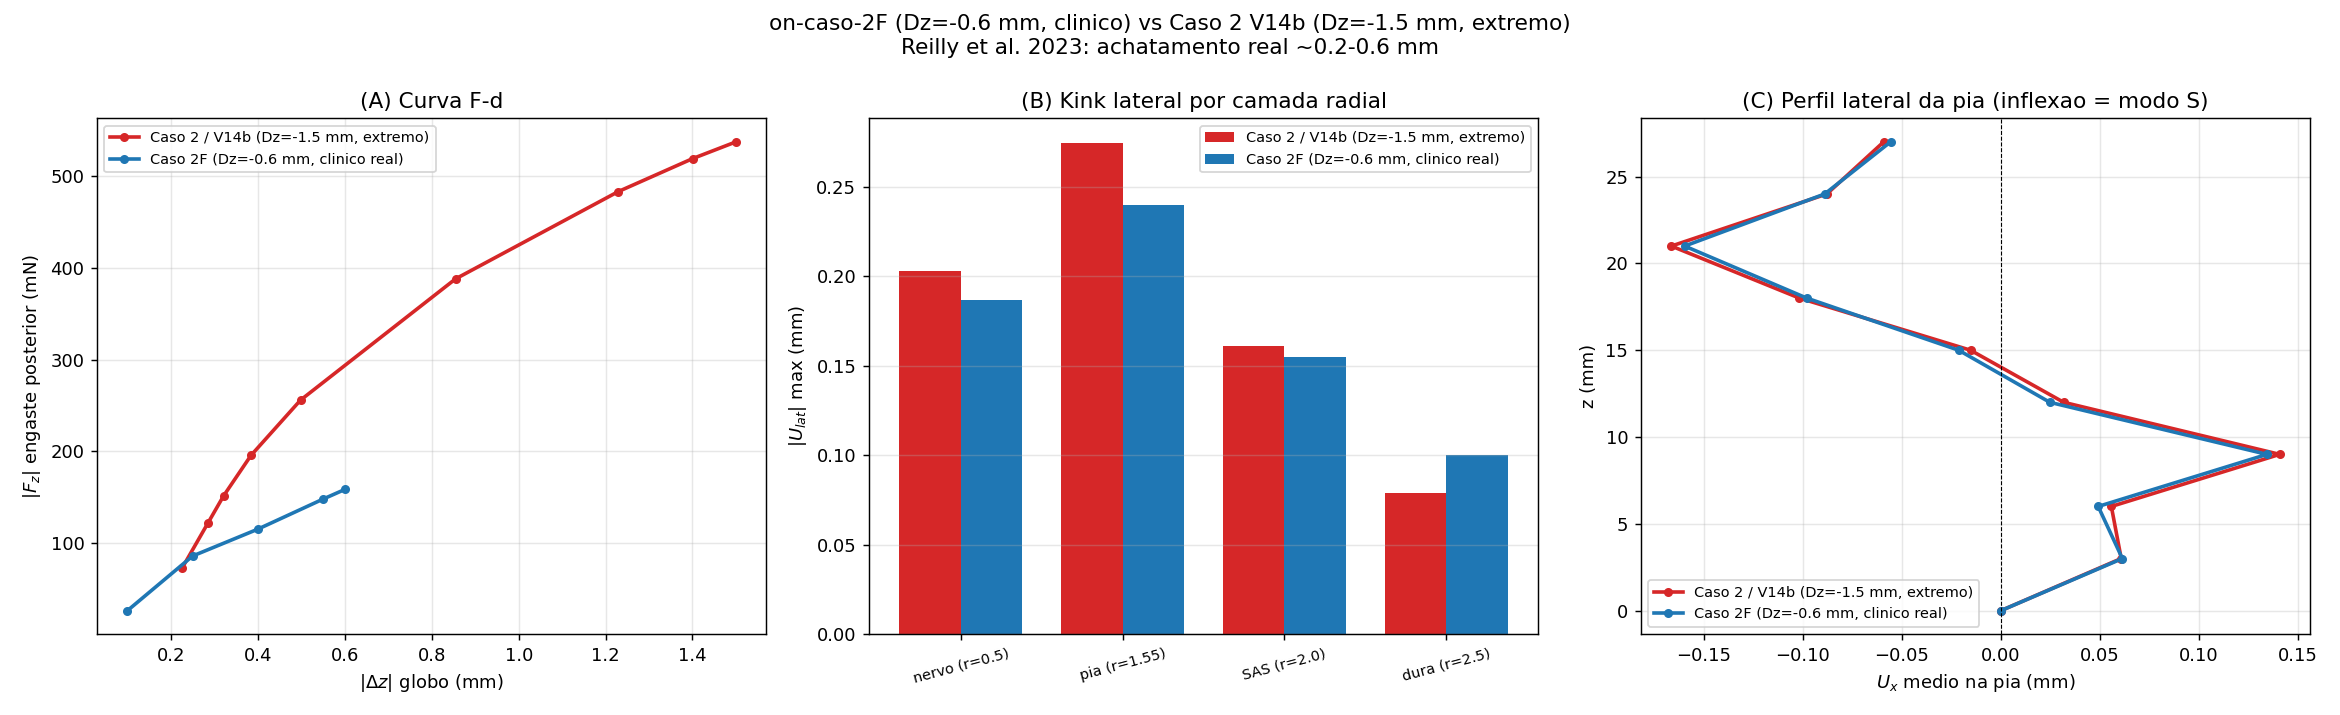
\includegraphics[width=0.85\linewidth]{on-caso-2F_comparacao.png}
% \caption{Caso 2F ($\Delta z = -\SI{0.6}{\milli\meter}$, clínico) versus caso 2
% ($\Delta z = -\SI{1.5}{\milli\meter}$, extremo): \emph{kink} lateral por camada.
% O modo S confinado (razão pia/dura $>1$) se mantém no deslocamento clínico.}
% \label{fig:res-caso2F}
% \end{figure}

% \subsection*{Caso 2g -- sensibilidade à rigidez da gordura orbital}
% \label{sec:res-caso2g}

% A varredura da fundação de Winkler de $k = \SI{20}{}$ a \SI{5000}{\kilo\pascal\per\meter} (gordura jovem $\to$ envelhecida/SANS) mostra que a rigidez da gordura modula a \emph{partição} da flambagem entre as camadas, mais do que a carga de engaste em si (Tabela~\ref{tab:res-caso2g}). Em fundação muito macia ($k = \SI{20}{\kilo\pascal\per\meter}$) a dura ainda acompanha parcialmente a deflexão (razão pia/dura $= 2.97$); ao endurecer a fundação a dura é progressivamente travada na parede, exceto pelo comportamento não-monotônico em $k = \SI{1}{\mega\pascal\per\meter}$, onde a mudança de modo aproxima as deflexões de pia e dura (razão $1.69$). Para a fundação SANS rígida ($k = \SI{5}{\mega\pascal\per\meter}$) a dura praticamente não dobra (razão $6.87$), concentrando toda a ondulação no tecido neural.

% \begin{table}[h!]
% \centering
% \small
% \caption{Caso 2g: força de engaste máxima e \emph{kink} por camada
% (\si{\milli\meter}) em função da rigidez de Winkler $k$.}
% \label{tab:res-caso2g}
% \begin{tabular}{l r r r r r r}
% \toprule
% $k$ (\si{\kilo\pascal\per\meter}) & $F_{\max}$ (\si{\milli\newton}) & nervo & pia & SAS & dura & pia/dura \\
% \midrule
% 20   & 792.1 & 0.176 & 0.226 & 0.141 & 0.076 & 2.97 \\
% 200  & 537.5 & 0.203 & 0.275 & 0.161 & 0.079 & 3.48 \\
% 1000 & 591.2 & 0.178 & 0.225 & 0.148 & 0.133 & 1.69 \\
% 5000 & 479.2 & 0.131 & 0.163 & 0.093 & 0.024 & 6.87 \\
% \bottomrule
% \end{tabular}
% \end{table}

% \begin{figure}[h!]
% \centering
% 
\includegraphics[width=0.85\linewidth]{on-caso-2g_sweep_winkler.png}
% \caption{Caso 2g: varredura da rigidez de Winkler $k$ e seu efeito sobre a
% flambagem por camada.}
% \label{fig:res-caso2g}
% \end{figure}

% \subsection*{Caso 2.2 -- tortuosidade anatômica (imperfeição em J)}
% \label{sec:res-caso2.2}

% Substituindo a perturbação artificial por uma curvatura real da linha de centro do nervo (imperfeição em J), a rigidez axial secante cai para $k_{\mathrm{axial}} \approx \SI{177}{\newton\per\meter}$ (Tabela~\ref{tab:res-malha}) -- cerca de $58\%$ da rigidez do nervo reto (\SI{305}{\newton\per\meter}). A folga anatômica funciona como imperfeição natural que reduz a carga necessária para iniciar a deflexão lateral, deslocando o eixo do nervo no plano $-y$ junto ao globo (Figura~\ref{fig:res-caso2.2}). Esse resultado valida o uso da tortuosidade real como gatilho da flambagem, em vez da perturbação numérica.

% \begin{figure}[h!]
% \centering
% 
\includegraphics[width=0.85\linewidth]{on-caso-2.2_tortuosity_slice.png}
% \caption{Caso 2.2: corte longitudinal da tortuosidade em J. A curvatura
% anatômica atua como imperfeição que reduz a rigidez axial efetiva.}
% \label{fig:res-caso2.2}
% \end{figure}

% \subsection*{Caso 3 -- contato da artéria oftálmica e mudança de modo}
% \label{sec:res-caso3}

% \paragraph{Varredura da pressão de contato.} Acrescentando ao caso~2 a pressão focal da artéria oftálmica em \texttt{contact\_local} ($+x$, $z \approx \SI{22.5}{\milli\meter}$) e varrendo $p_c = 0 \to \SI{18068}{\pascal}$, a Tabela~\ref{tab:res-caso3sweep} mostra duas respostas combinadas. Primeiro, a deflexão lateral da dura cresce monotonicamente ($\mathrm{kink}_{\mathrm{dura}}$ de \SI{0.066}{} a \SI{0.830}{\milli\meter}), agora forçada a dobrar pela carga focal externa. Segundo, a partir de $p_c = \SI{13551}{\pascal}$ a estrutura não suporta mais a carga lateral total: o fator de Riks satura ($\lambda < 1$, descendo a $0.65$ em $p_c = \SI{18068}{\pascal}$) e a carga máxima atingível cai (\emph{snap}/colapso), assinatura do agravamento do dobramento pela artéria.

% \begin{table}[h!]
% \centering
% \small
% \caption{Caso 3: varredura da pressão de contato arterial $p_c$. $\lambda$ é o
% fator de Riks máximo atingido; $\mathrm{Ur}_{\min}$ a compressão radial máxima
% na pegada.}
% \label{tab:res-caso3sweep}
% \begin{tabular}{r c r r r r}
% \toprule
% $p_c$ (\si{\pascal}) & $\lambda$ & $F_{\max}$ (\si{\milli\newton}) & $\mathrm{kink}_{\mathrm{on}}$ & $\mathrm{kink}_{\mathrm{dura}}$ & $\mathrm{Ur}_{\min}$ (\si{\milli\meter}) \\
% \midrule
% 0      & 1.00 & 731.8 & 0.171 & 0.066 & $-0.049$ \\
% 4517   & 1.00 & 331.3 & 0.364 & 0.386 & $-0.386$ \\
% 9034   & 1.00 & 328.6 & 0.467 & 0.694 & $-0.694$ \\
% 13551  & 0.73 & 145.4 & 0.307 & 0.594 & $-0.594$ \\
% 18068  & 0.65 & 135.2 & 0.357 & 0.830 & $-0.830$ \\
% \bottomrule
% \end{tabular}
% \end{table}

% \paragraph{Fechamento do espaço subaracnoide.} A pressão de contato comprime radialmente a bainha e estreita o SAS: a folga dura--pia, inicialmente \SI{0.80}{\milli\meter}, reduz-se $31.4\%$ em $p_c = \SI{9034}{\pascal}$, $53.0\%$ em \SI{13551}{\pascal} e $79.1\%$ em \SI{18068}{\pascal} (\texttt{dura\_pia\_gap}). Esse colapso quase total do espaço perineural sob carga arterial sistólica reproduz o estrangulamento focal observado na SANS.

% \paragraph{Mudança de modo crítico (Hetényi).} A variante SANS com fundação rígida ($k_w = \SI{2}{\mega\pascal\per\meter}$, caso~3) muda o modo crítico de Hetényi de $n = 1$ ($\lambda = \SI{30}{\milli\meter}$, $P_{\mathrm{cr}} = \SI{507.8}{\milli\newton}$, saudável) para $n = 2$ ($\lambda = \SI{15}{\milli\meter}$, $P_{\mathrm{cr}} = \SI{1601}{\milli\newton}$), um aumento de $3.15\times$ na carga crítica. Embora a rigidez axial total seja praticamente idêntica à do caso saudável ($+0.29\%$, pois o Winkler não resiste à compressão axial), a transição $n=1 \to n=2$ significa que o nervo passa de um arco suave para uma \emph{ondulação focal} de duas meias-ondas -- exatamente o padrão clínico da SANS: pontos de estrangulamento em vez de uma curvatura difusa.

% \subsection*{Caso 3-sf / 3-inv -- isolamento e simetria de espelho do contato}
% \label{sec:res-caso3sf}

% Removendo a compressão frontal do globo (sem $\Delta z$, sem EOM) para isolar \emph{só} a artéria, a deflexão lateral do nervo cai de \SI{449}{\micro\meter} (caso~3 completo) para \SI{334.8}{\micro\meter} (\texttt{3-sf}). A variante espelhada (\texttt{3-inv}, contato em $-x$) produz \SI{330.2}{\micro\meter}, com o nervo defletindo para o lado oposto -- diferença de apenas $1.4\%$ em amplitude, confirmando que o modo de deformação é \emph{simétrico} em relação ao hemisfério de contato e governado pela física, não por viés numérico (Tabela~\ref{tab:res-caso3sf}). Note-se ainda que, sem a compressão axial, a amplitude de \emph{span} axial cai de \SI{1499}{} para $\sim\SI{10}{\micro\meter}$ e desaparecem os cortes de passo do Riks (de 2 para 0), indicando que a carga arterial isolada é bem-comportada numericamente.

% \begin{table}[h!]
% \centering
% \small
% \caption{Caso 3 -- isolamento e espelhamento do contato arterial
% ($p_c = \SI{9034}{\pascal}$).}
% \label{tab:res-caso3sf}
% \begin{tabular}{l r c r}
% \toprule
% \textbf{Variante} & $|U_x|_{\max}$ (\si{\micro\meter}) & lado & \emph{span} axial (\si{\micro\meter}) \\
% \midrule
% \texttt{caso-3} (completo, $+x$) & 449.0 & $-x$ & 1498.8 \\
% \texttt{caso-3-sf} (só artéria, $+x$) & 334.8 & $-x$ & 10.2 \\
% \texttt{caso-3-inv} (só artéria, $-x$) & 330.2 & $+x$ & 10.5 \\
% \bottomrule
% \end{tabular}
% \end{table}

% \subsection*{Caso 4 -- inchaço da bainha acopla área e força de contato}
% \label{sec:res-caso4}

% O caso~4 fecha o raciocínio da SANS: em vez de uma carga arterial fixa, a área e a força de contato são \emph{derivadas} do inchaço da bainha, ele próprio dirigido pela PIC. A Fase~A mede a expansão radial da dura $\Delta r$ em função da PIC; a Fase~B converte essa interferência em pegada de contato (caixa \texttt{topoSet} ampliada) e pressão $p_c = k_{\mathrm{art}}\,\delta$ ($k_{\mathrm{art}} = \SI{3.197e9}{\pascal\per\meter}$). A Tabela~\ref{tab:res-caso4} reporta os quatro estágios de SANS.

% \begin{table}[h!]
% \centering
% \small
% \caption{Caso 4: resposta acoplada inchaço$\to$contato por estágio de SANS.
% $\Delta r$: expansão radial da dura (Fase A); $A$: área da pegada; $p_c$/$F$:
% pressão e força de contato; \emph{kink}/offset: deflexão lateral;
% $\sigma_{\mathrm{vM}}$: von Mises de pico.}
% \label{tab:res-caso4}
% \begin{tabular}{l r r r r r r r r}
% \toprule
% \textbf{Estágio} & \makecell{P\textsubscript{LCR}\\(\si{\pascal})} & \makecell{$\Delta r$\\(\si{\micro\meter})} & \makecell{$A$\\(\si{\milli\meter\squared})} & \makecell{$p_c$\\(\si{\pascal})} & \makecell{$F$\\(\si{\milli\newton})} & \makecell{kink\\(\si{\milli\meter})} & \makecell{offset\\(\si{\milli\meter})} & \makecell{$\sigma_{\mathrm{vM}}$\\(\si{\kilo\pascal})} \\
% \midrule
% S0 (basal, \SI{10}{mmHg}) & 1333 & 2.83  & 3.93  & 9034  & 35.5  & 0.093 & 0.084 & 110.0 \\
% S1 (leve, \SI{18}{mmHg})  & 2400 & 5.11  & 11.78 & 16333 & 192.4 & 0.438 & 0.413 & 698.3 \\
% S2 (upper, \SI{28}{mmHg}) & 3800 & 8.05  & 19.64 & 18068 & 354.8 & 0.685 & 0.657 & 601.1 \\
% S3 (severo, \SI{41}{mmHg}) & 5500 & 11.58 & 23.56 & 18068 & 425.7 & 0.731 & 0.711 & 470.5 \\
% \bottomrule
% \end{tabular}
% \end{table}

% A expansão radial cresce de \SI{2.83}{} a \SI{11.58}{\micro\meter} (fator $4.1\times$) e arrasta consigo a área de contato ($3.93 \to \SI{23.56}{\milli\meter\squared}$) e a força ($35.5 \to \SI{425.7}{\milli\newton}$), confirmando o acoplamento inchaço$\to$contato hipotetizado. O deslocamento lateral do nervo (\emph{kink} e offset) cresce monotonicamente até $\sim\SI{0.7}{\milli\meter}$ em S3. Já a tensão de von Mises de pico \emph{não} é monotônica: atinge o máximo em S1 (\SI{698}{\kilo\pascal}) e depois decai (S2 \SI{601}{}, S3 \SI{470}{\kilo\pascal}), porque a partir de S1 a pressão de contato satura no valor sistólico (\SI{18068}{\pascal}) e a carga passa a se distribuir sobre uma pegada cada vez maior, reduzindo a concentração local mesmo com força total crescente (Figura~\ref{fig:res-caso4}). Esse achado tem implicação clínica: o pico de insulto tensional ocorre num estágio \emph{intermediário} da progressão, não no mais severo.

% \begin{figure}[h!]
% \centering
% 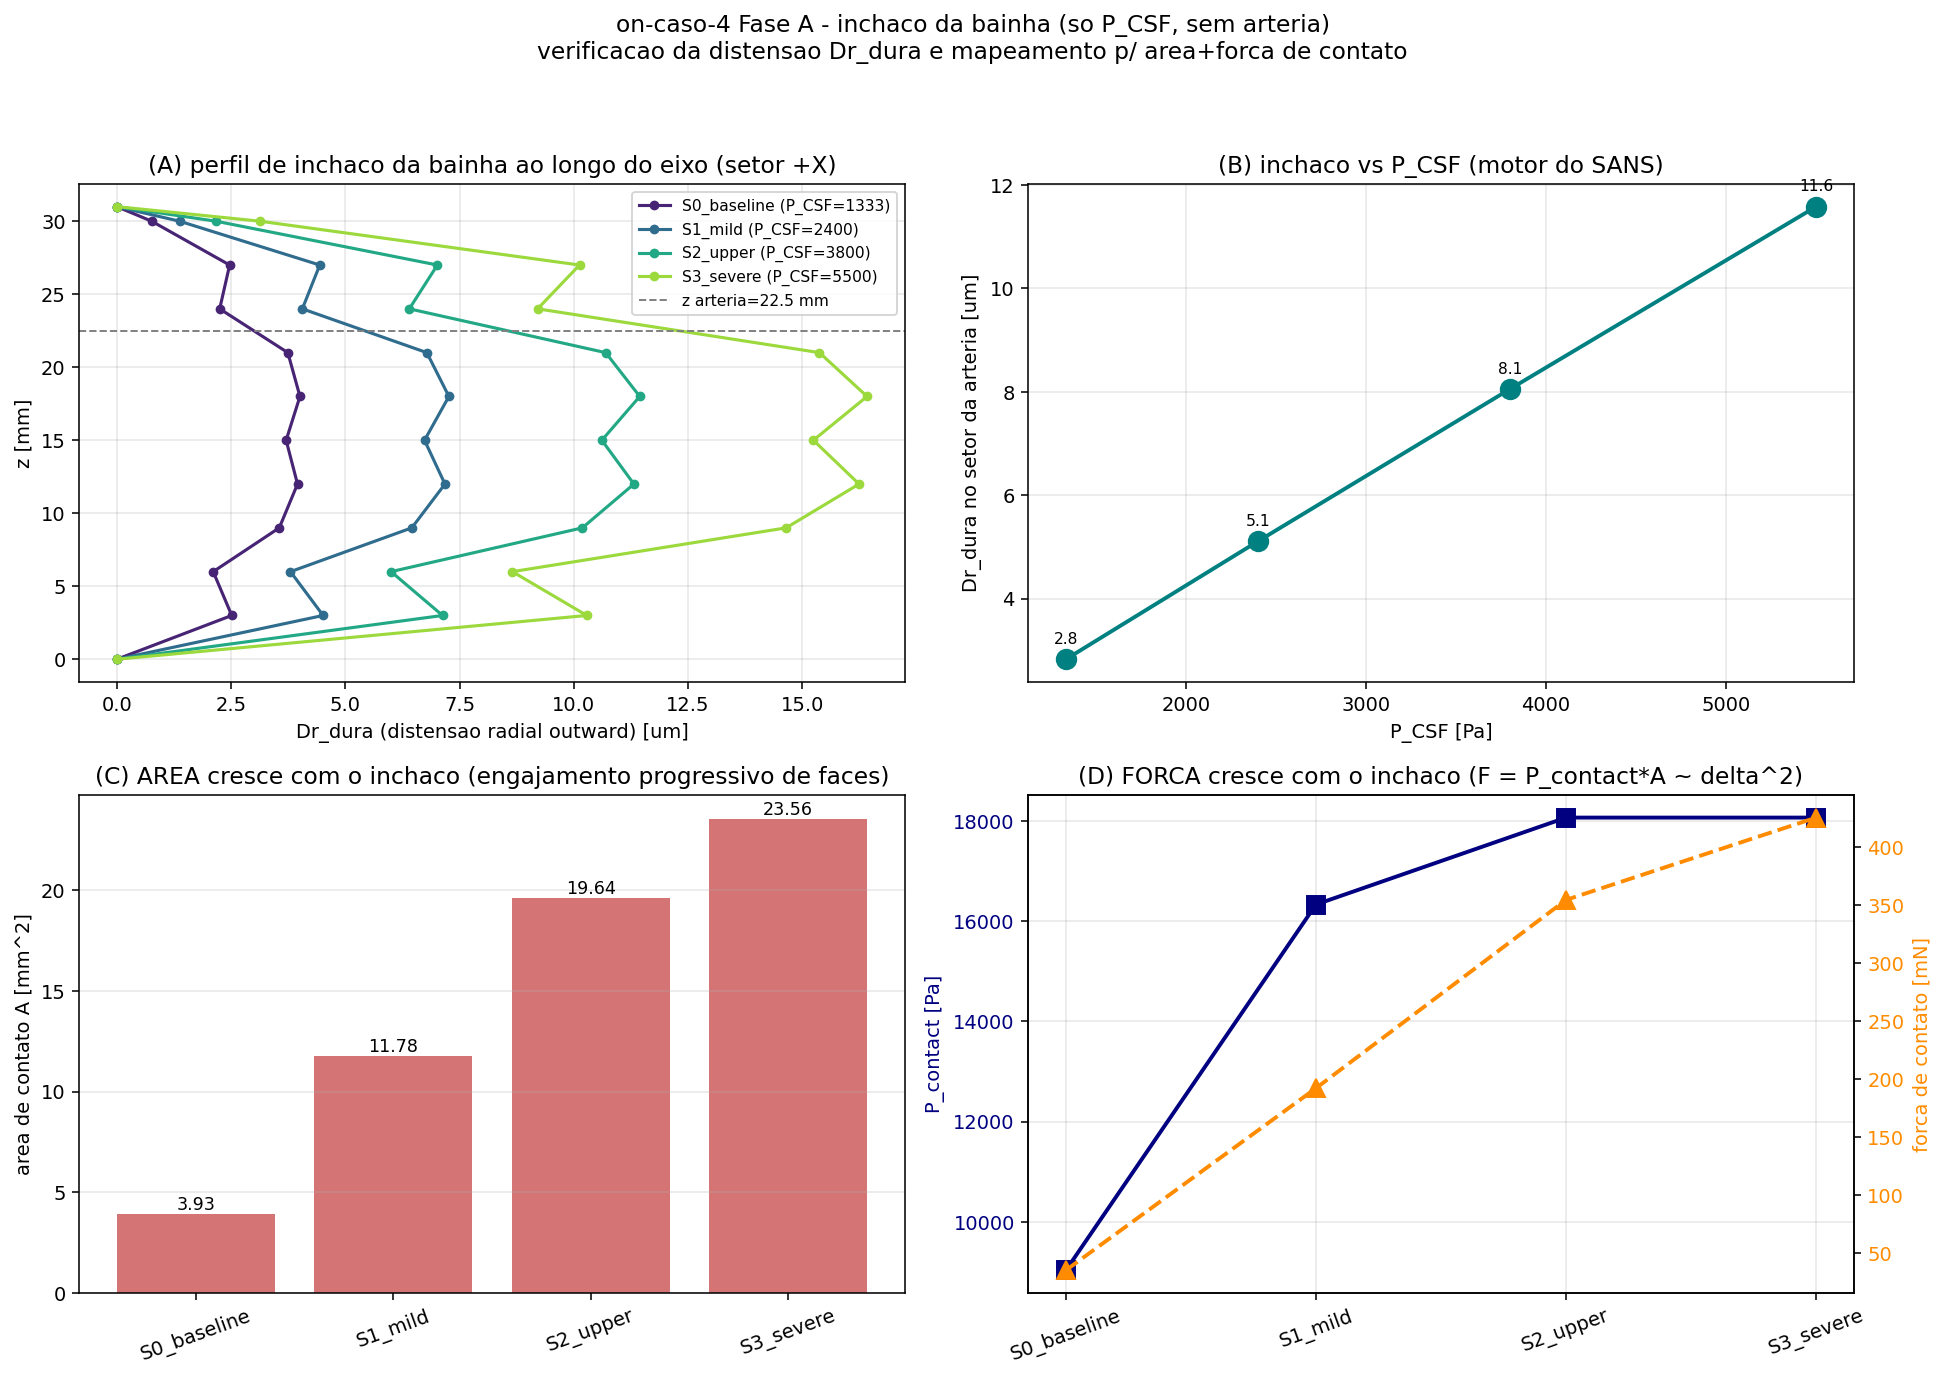
\includegraphics[width=0.49\linewidth]{on-caso-4_swelling.png}
% 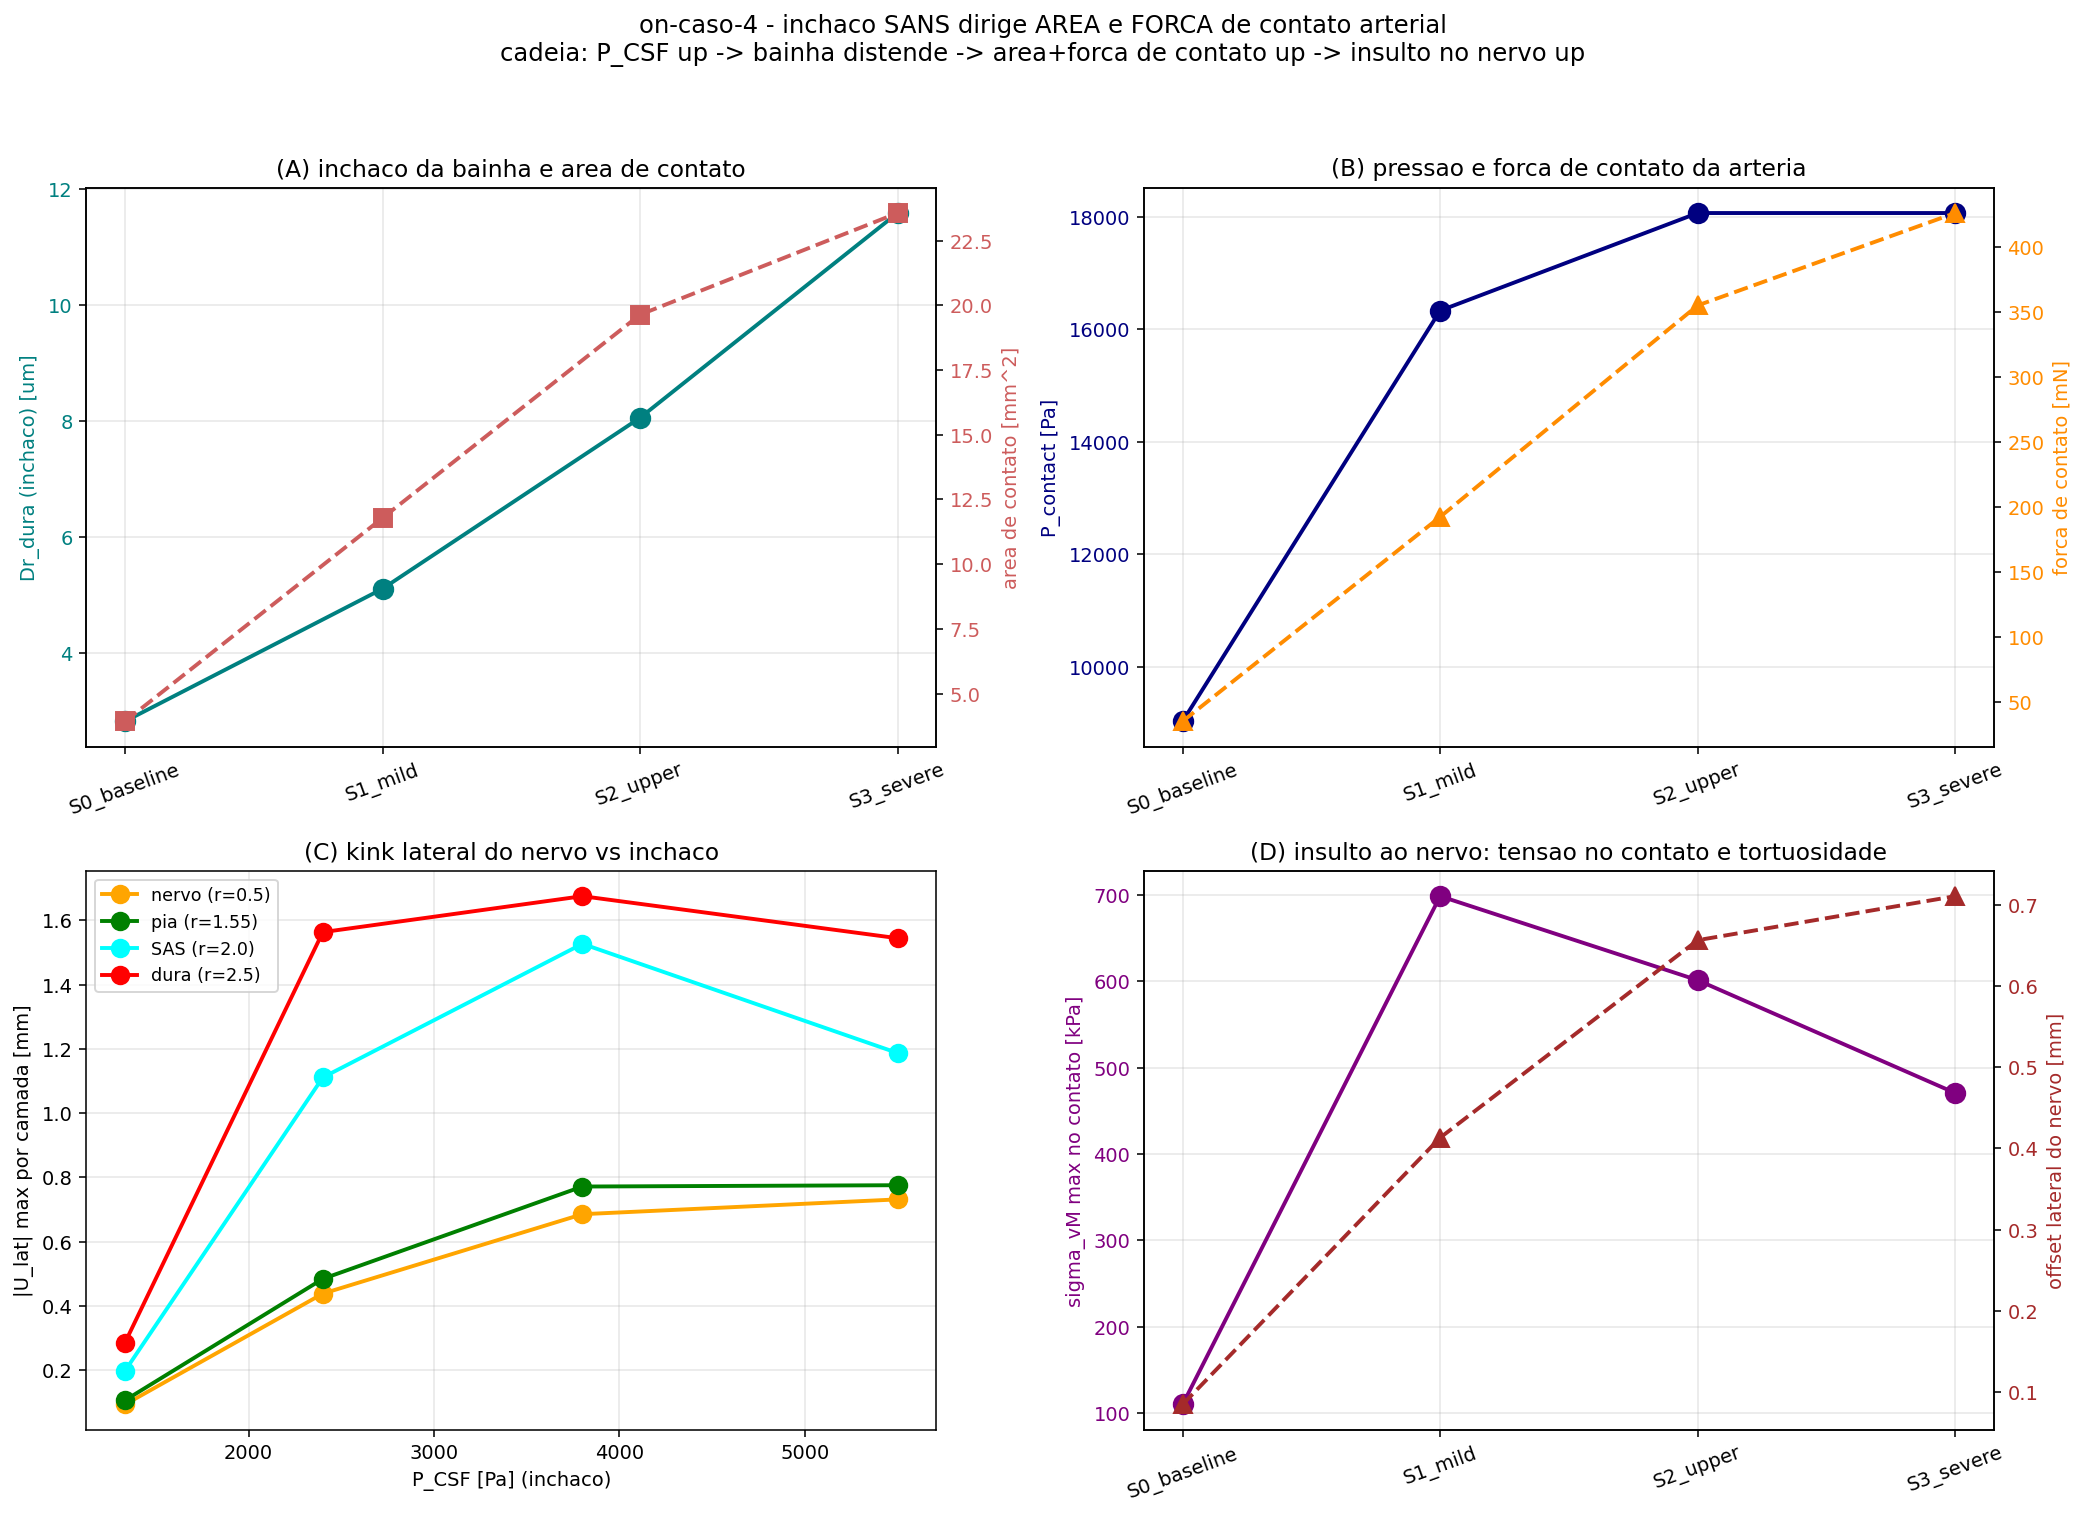
\includegraphics[width=0.49\linewidth]{on-caso-4_summary.png}
% \caption{Caso 4. \emph{Esquerda:} expansão radial da bainha $\Delta r$ por
% estágio (Fase A). \emph{Direita:} resposta acoplada -- área, força e von Mises
% de pico em função do estágio de SANS.}
% \label{fig:res-caso4}
% \end{figure}

% \subsection*{Caso 1.2 -- FSI com drenagem porosa e compartimentalização}
% \label{sec:res-fsi}

% O caso FSI \texttt{on-caso-1.2} (LCR resolvido pelo \texttt{pimpleFluid}, estrutura no CalculiX, acoplamento preCICE) quantifica a compartimentalização do LCR pela resistência hidráulica do \emph{lid} poroso de drenagem (Darcy--Forchheimer, coeficiente $d$). Dois modos foram estudados.

% \paragraph{Modo pressão prescrita (varredura de Darcy).} Com pressão fixa no \emph{inlet} e saída livre, a varredura $d \in \{10^{13};\,10^{15};\,10^{17}\}\, \si{\per\meter\squared}$ produz escalamento de Darcy puro: a vazão de drenagem $Q$ cai de \SI{9.96e-10}{} (\emph{lid} aberto) a \SI{9.96e-14}{\meter\cubed\per \second} (compartimentalização tipo IIH/SANS), passando pelo regime fisiológico saudável $\sim\SI{1e-11}{\meter\cubed\per\second}$ em $d = \SI{1e15}{\per\meter \squared}$. Como as pressões de contorno estão ancoradas, a compartimentalização se manifesta no \emph{fluxo} (cai $100\times$ por década de $d$), mapeando diretamente a obstrução das vilosidades aracnoides perineurais \citep{Killer2003, Mathieu2017, Wostyn2017}.

% \paragraph{Modo PIC-driven (vazão prescrita).} Substituindo o \emph{inlet} por vazão fisiológica fixa ($Q_{\mathrm{in}} = \SI{3e-11}{\meter\cubed\per\second}$), qualquer aumento de $d$ exige elevação proporcional da pressão no SAS \emph{bulk} -- exatamente a hipótese SANS. A Tabela~\ref{tab:res-fsi} mostra a transição: a PIC no \emph{bulk} passa de regime aberto (negativo, dominado por Bernoulli transiente) ao saudável ($\sim\SI{1106}{\pascal} \approx$ PIC basal de \SI{1333}{\pascal}) em $d = \SI{1e15}{}$, e salta para $\sim\SI{14039}{\pascal}$ ($\sim\SI{105}{mmHg}$, hipertensão intracraniana severa) em $d = \SI{1e16}{\per\meter\squared}$. A transição saudável$\to$severo ocorre num único \emph{decade} de $d$ (fator $12.7\times$ em PIC), consistente com a observação clínica de que pequenas variações na permeabilidade das vias de drenagem disparam a compartimentalização do ONSAS.

% \begin{table}[h!]
% \centering
% \small
% \caption{Caso 1.2, modo PIC-driven: PIC no \emph{bulk} e queda de pressão no
% \emph{lid} em função do coeficiente de Darcy $d$.}
% \label{tab:res-fsi}
% \begin{tabular}{r r r l}
% \toprule
% $d$ (\si{\per\meter\squared}) & $\mathrm{PIC}_{\mathrm{bulk}}$ (\si{\pascal}) & $\Delta p_{\mathrm{lid}}$ (\si{\pascal}) & Regime \\
% \midrule
% $10^{12}$ & $-330$  & $-85$  & \emph{lid} aberto (Bernoulli) \\
% $10^{13}$ & $-317$  & $-81$  & idem \\
% $10^{14}$ & $-188$  & $-36$  & quase aberto \\
% $10^{15}$ & $1106$  & $410$  & \textbf{saudável} ($\sim$PIC basal) \\
% $10^{16}$ & $14039$ & $4871$ & \textbf{IIH/SANS severo} ($\sim$\SI{105}{mmHg}) \\
% \bottomrule
% \end{tabular}
% \end{table}

% \begin{figure}[h!]
% \centering
% 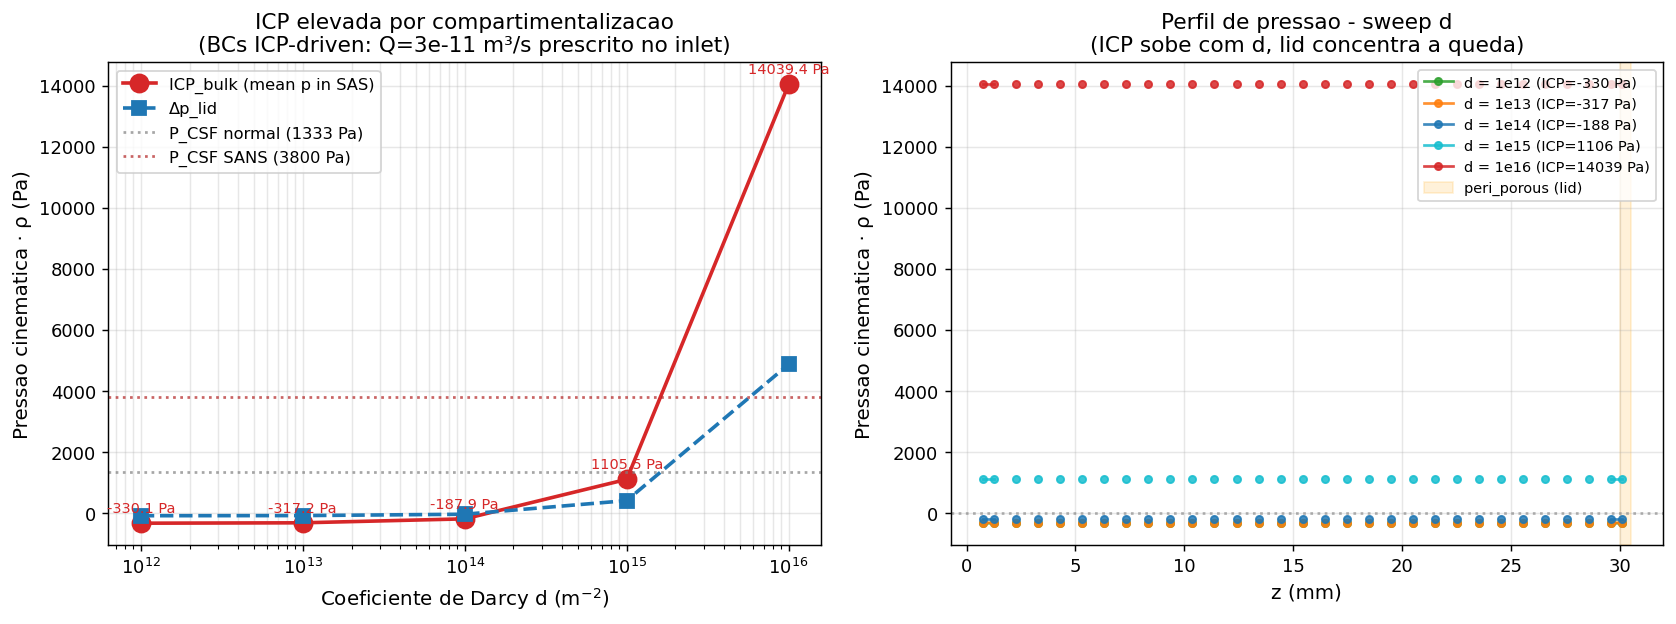
\includegraphics[width=0.85\linewidth]{figs/on-caso-1.2-pic-driven.png}
% \caption{Caso 1.2 (FSI, modo PIC-driven): PIC no \emph{bulk} do SAS em função do
% coeficiente de Darcy $d$ e perfil de pressão $p(z)$ ao longo do eixo do nervo. A
% transição saudável$\to$SANS-severo ocorre numa única década de $d$.}
% \label{fig:res-fsi}
% \end{figure}

% \paragraph{\emph{Caveat} numérico.} O acoplamento FSI completo com material Neo-Hookeano colapsa para $\mathrm{PIC}_{\mathrm{bulk}} > \SI{1500}{\pascal}$ ($d \ge \SI{1e15}{\per\meter\squared}$ no modo PIC-driven), por divergência do Newton--Raphson do CalculiX: as forças FSI excedem a capacidade portante das lâminas pia/dura no regime hiperelástico. O regime severo da Tabela~\ref{tab:res-fsi} foi, portanto, obtido no caso auxiliar \emph{fluid-only} (\texttt{on-caso-1.2-fluidonly}, mesma malha e \texttt{fvOptions}, sem o lado estrutural). A extensão para o acoplamento completo sob PIC elevada requer \emph{ramping} de carga multi-step ou amortecimento, e é trabalho futuro.

% \subsection*{Discussão integradora: o mecanismo da SANS}
% \label{sec:res-discussao}

% A progressão dos casos sustenta um mecanismo coerente para a SANS. O caso~2 estabelece que o complexo nervo+pia flamba em modo S confinado, com a dura respondendo por $\sim 77\%$ da rigidez axial e a flambagem de Euler clássica \emph{descartada} como modo de falha ($F_z/P_{\mathrm{cr}} \le 60\%$ em $K \le 0.65$). O caso~2F mostra que esse esmagamento neural já ocorre em deslocamentos clínicos (\SI{-0.6}{\milli\meter}), e o caso~2.2 que a tortuosidade anatômica reduz em $\sim 42\%$ a rigidez efetiva, atuando como gatilho natural. O achado mais relevante para a fenomenologia clínica é a \emph{mudança de modo crítico} entre o caso saudável e o SANS (caso~3): o endurecimento da gordura orbital ($k_w$: \SI{200}{\kilo\pascal\per\meter} $\to$ \SI{2}{\mega\pascal\per \meter}) desloca o modo de Hetényi de $n=1$ (arco difuso) para $n=2$ (ondulação focal de $\lambda = \SI{15}{\milli\meter}$), reproduzindo o padrão de estrangulamento focal observado em ressonância. O contato arterial (caso~3) fecha o SAS em até $79\%$ sob carga sistólica, e o caso~4 demonstra que o próprio inchaço da bainha, dirigido pela PIC, intensifica de forma acoplada a área e a força do contato -- com o pico de insulto tensional num estágio intermediário (S1) por saturação da pressão de contato. Finalmente, o caso FSI~1.2 fornece o elo causal a montante: a obstrução das vias de drenagem perineural (coeficiente de Darcy $d$) eleva a PIC no \emph{bulk} de forma abrupta numa única década de $d$, ligando a fisiopatologia da drenagem ao carregamento mecânico que dispara toda a cascata estrutural.

% \subsection*{Limitações}
% \label{sec:res-limitacoes}

% Os casos estruturais são quase-estáticos e não capturam a pulsação arterial transiente sobre uma bainha pré-tensionada, hipótese central para a tortuosidade dinâmica. As leis constitutivas, embora Neo-Hookeanas (grandes deformações), não incorporam a anisotropia de fibras de colágeno da pia e da dura \citep{Holzapfel2000}, relevante acima de $\sim 5\%$ de deformação. O acoplamento FSI completo (caso~1.2) não converge sob PIC $> \SI{1500}{\pascal}$ no regime hiperelástico, restringindo o mapeamento PIC-driven severo ao caso \emph{fluid-only}. A artéria oftálmica é representada como carga de contato prescrita, não como fluido acoplado (acoplamento de três vias), e a pressão intraocular não é modelada -- de modo que os indicadores reportados representam um limite do efeito da PIC isolada sobre o segmento intraorbitário.









% %%%%%%%%%%%%%%%%%%%%%%%%%%%%%%%%%%%%%%%%%%%%%%%%%%%%%%%%%%%%%%%%%%%%%%%%%%%%%%%%%%%%%%%
% %%%%%%%%%%%%%%%%%%%%%%%%%%%%%%%%%%%%%%%%%%%%%%%%%%%%%%%%%%%%%%%%%%%%%%%%%%%%%%%%%%%%%%%
% %%%%%%%%%%%%%%%%%%%%%%%%%%%%%%%%%%%%%%%%%%%%%%%%%%%%%%%%%%%%%%%%%%%%%%%%%%%%%%%%%%%%%%%
% %%%%%%%%%%%%%%%%%%%%%%%%%%%%%%%%%%%%%%%%%%%%%%%%%%%%%%%%%%%%%%%%%%%%%%%%%%%%%%%%%%%%%%%
% %%%%%%%%%%%%%%%%%%%%%%%%%%%%%%%%%%%%%%%%%%%%%%%%%%%%%%%%%%%%%%%%%%%%%%%%%%%%%%%%%%%%%%%


% \section*{Conclusões}
% \label{sec:conclusoes}

% A representação do LCR como fluido é necessária: o FSI reproduz o princípio de Pascal e revela seu papel amortecedor isotrópico, enquanto o modelo puramente estrutural é qualitativamente insensível à pressão intracraniana \citep{Lee2020NPJ, Mader2011, Chourdakis2022}.

% A flambagem axial clássica de Euler não é modo de falha relevante na faixa clínica do \emph{shift} cefálico (margem $\sim 2.4\times$), e a compartimentalização do espaço subaracnoide do nervo óptico ocorre num único \emph{decade} do coeficiente de obstrução da drenagem (detalhamento na Seção~\ref{sec:resultados-sans}).

% As conclusões valem sob regime estático, artéria como pressão prescrita e leis lineares, de modo que a continuidade natural passa pelo FSI transiente, por hiperelasticidade anisotrópica \cite{Holzapfel2000} e pela inclusão do gradiente de pressão translaminar.

\newpage


\bibliography{ref.bib}

\end{document}



